% !TeX program = lualatex
% !TeX encoding = utf8
% !TeX spellcheck = uk_UA
% !BIB program = biber

\documentclass{LabWork}
%\usepackage{fixfoot}
%\usepackage{minted}

%\DeclareFixedFootnote{\repnote}{\fullcite{Spavieri2004}}
\addbibresource{LabWork1.bib}
\graphicspath{{LabWork1pic/}}
\usetikzlibrary{arrows.meta}
\tikzset{
every info/.style={font=\small},
}
\newcommand\Ground{%
\mathbin{\text{\begin{tikzpicture}[circuit ee IEC]
\draw (0,1ex) to (0,0) node[ground,rotate=-90,xshift=.3ex] {};
\end{tikzpicture}}}%
}

%============================================= Заголовок документу ====================================================%
\work{1}
\title{Перевірка закону Кулона}

%\author{Тор А.~В.}{}
%\author{Другий А.~В.}{}

%\group{ФФ-93}

\abstract{%

Перевірити закон Кулона:
\begin{enumerate}
\item Визначити залежність сили від заряду;
\item визначити залежність сили від відстані;
\item визначити електричну сталу в системі SI.
\end{enumerate}
}
%======================================================================================================================%

\begin{document}
\writedatatofile{\jobname}
\maketitle

\section{Теоретичні відомості}

З давніх-давен відоме явище електризації тіл тертям. Якщо потерти скляну або гумову паличку, вона притягуватиме шматочки паперу з силою, яка достатня для подолання їх ваги. Як ми тепер знаємо, завдяки тертю паличка набуває електричного заряду. Незважаючи на велику кількість різних речовин, в природі існують тільки два види електричних зарядів: заряди подібні тим, які виникають на склі, потертому об шовк, і заряди, подібні до тих, які з'являються на бурштині, потертому об хутро. Американський вчений Бенджамін Франклін у 1746 р. перший тип зарядів назвав <<позитивними>>, другий --- <<негативними>>.  В взаємодія двох таких зарядів один з одним подібна до притягування двох мас. Але на відміну від сил тяжіння, сили між двома зарядами можуть носити характер не лише притягування, а і відштовхування. Порівнюючи сили, що діють між різними зарядженими тілами, можна встановити, що однойменні заряди відштовхуються, а різнойменні притягують один одного. Точний закон взаємодії заряджених тіл було відкрито Шарлем Огюстеном Кулоном\footnote{На початку 1770-х років цей закон експериментально відкрив Генрі Кавендіш, однак своїх результатів він не опублікував, і про них стало відомо тільки в кінці XIX ст. після вивчення й публікації його архівів. Натомість Шарль Кулон опублікував закон в двох мемуарах у 1785 році,  які представив на розгляд Французької академії наук.} в результаті експериментів і формулюється він наступним чином:

\begin{tcolorbox}
Сила взаємодії двох точкових зарядів у вакуумі направлена вздовж прямої, що з'єднує ці заряди, пропорційна добутку їх величин і обернено пропорційна квадрату відстані між ними. Ця сила носить характер притягування, якщо знаки зарядів різні, і відштовшування --- якщо ці знаки однакові.
\end{tcolorbox}

У векторному вигляді закон Кулона записується наступним чином:

\begin{equation}\label{key}
    \tcbhighmath[drop fuzzy shadow]{
    \vec{F}_{12}=k\cdot\frac{q_1  q_2}{r_{12}^2} \cdot \frac{\vec{r}_{12}}{r_{12}},
    }
\end{equation}
де $\vec{F}_{12}$ --- сила, p якою заряд $1$ діє на заряд $2$; $q_1$, $q_2$ --- величини зарядів; $\vec{r}_{12}$ --- вектор, напрямлений від заряду $1$ до заряду  $2$ і за модулем дорівнює відстані між зарядами; $k$ --- коефіцієнт пропорційності, який залежить від вибору системи одиниць. 

Для того, щоб закон був справедливим, необхідно, щоб виконувались наступні умови:
\begin{enumerate}
\item заряди мають бути точковими, тобто відстань між зарядженими тілами повинна бути набагато більша за їх розміри. Однак, на основі теореми Гауса можна довести, що сила взаємодії однорідно заряджених куль дорівнює силі взаємодії еквівалентних точкових зарядів, що розташовуються в центрах цих куль;
\item заряди мають бути нерухомі;
\item заряди мають знаходитись у вакуумі.
\end{enumerate}

\begin{wrapfigure}{l}{0.5\linewidth}\centering
	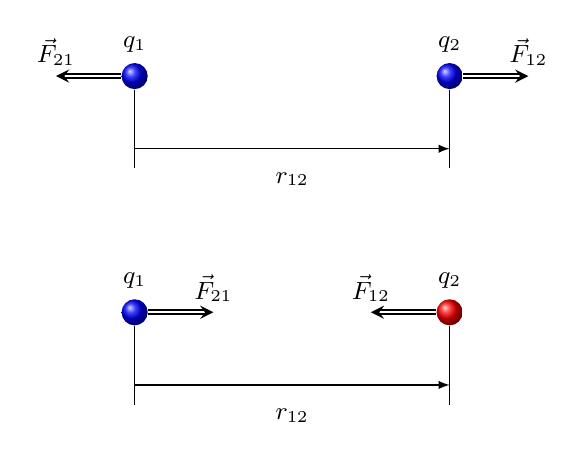
\begin{tikzpicture}[scale=1, font=\small,
						bodyb/.style={ball color=blue, circle},
                        bodyr/.style={ball color=red, circle},
                        fw/.style={fill=white, inner sep=1pt},
					]
					\node[bodyb] (q1) at (-2,0) {}; \node[above=5pt] at (q1) {$q_1$};
					\node[bodyb] (q2) at (2,0) {}; \node[above=5pt] at (q2) {$q_2$};
                    \draw (q1.south) -- coordinate[pos=0.75] (A) +(0,-1);
                    \draw (q2.south) -- coordinate[pos=0.75] (B) +(0,-1);
                    \draw[black, -latex]   (A) -- node[below=5pt]            {$r_{12}$} (B);
                    \draw[-stealth, double, thick] (q2) -- +(1,0) node[above] {$\vec{F}_{12}$};
                    \draw[-stealth, double, thick] (q1) -- +(-1,0) node[above] {$\vec{F}_{21}$};
                    \begin{scope}[yshift=-3cm]
    					\node[bodyb] (q1) at (-2,0) {}; \node[above=5pt] at (q1) {$q_1$};
    					\node[bodyr] (q2) at (2,0) {}; \node[above=5pt] at (q2) {$q_2$};
                        \draw (q1.south) -- coordinate[pos=0.75] (A) +(0,-1);
                        \draw (q2.south) -- coordinate[pos=0.75] (B) +(0,-1);
                        \draw[black, -latex]   (A) -- node[below=5pt]            {$r_{12}$} (B);
                        \draw[-stealth, double, thick] (q2) -- +(-1,0) node[above] {$\vec{F}_{12}$};
                        \draw[-stealth, double, thick] (q1) -- +(+1,0) node[above] {$\vec{F}_{21}$};
                    \end{scope}
	\end{tikzpicture}
	\caption{}
	\label{thpic1}
\end{wrapfigure}
Відкриття закону Кулона вперше дозволило розглядати заряд як певну кількість --- вимірювати його. В законі Кулона ми маємо право вибрати одиницю виміру за власним уподобанням і покласти $ k = 1$. Так, в системі СГС, одиничний заряд діє на рівний йому заряд на відстані в $1$~см з силою в одну дину (дина є сила, яка збільшує швидкість тіла з масою в $1$~г на $1$ см/с$^2$). Одиниця заряду, встановлена таким чином називається \emph{Франкліном} (Фр).

В практичній системі одиниць SI, заряд вимірюють в \emph{Кулонах} (Кл). Кулон є похідною одиницею системи SI і через основні одиниці Ампер (А) та секунду (с) визначається як $1$~Кл = $1$~А $\cdot$ $1$~с. В цій системі одиниць константа в законі Кулона дорівнює значенню $k = 8.9875 \cdot 10^{9} \approx 9\cdot 10^{9}$~$\frac{\text{Н}\cdot\text{м}^2}{\text{Кл}^2}$. В теорії електромагнітного поля в системі SI цю константу прийнято представляти через іншу константу у вигляді:
\begin{equation}\label{}
    k = \frac{1}{4\pi\varepsilon_0},
\end{equation}
де $\varepsilon_0 = 8.85418782 \cdot 10^{-12}$~$\frac{\text{А}^2\cdot\text{с}^4}{\text{м}^3\cdot\text{кг}}$ і називається електричною сталою.


%Закон Кулона дуже подібний за своєю математичною формою до закону Всесвітнього тяжіння. При цьому роль мас відіграють електричні заряди.

Однією важливою особливістю кулонівської взаємодії є її величина. Елек\-тричні сили між окремими елементарними частинками набагато більше гравітаційних. Якби вдалося передати 1\% електронів
від однієї людини іншій, то на відстані витягнутої руки сила тяжіння між ними перевищувала б вагу Земної кулі.  Взаємодія між зарядженими частинками настільки велика, що створити у невеликого тіла дуже великий заряд неможливо. Відштовхуючись один від одного з великою силою, частинки не зможуть утриматися на тілі. Ніяких же інших сил, які були б здатні в даних умовах компенсувати кулонівське відштовхування, в природі не існує. Ось одна з причин, чому помітне притягання та відштовхування заряджених тіл не зустрічається в природі. Крім того, заряджені тіла проявляють дуже велику схильність до нейтралізації. Вони з великою жадібністю вбирають заряди протилежного знака, притягаючи їх до себе. Більшість тіл в природі електрично нейтральні. Втім, сама Земля має негативний заряд близько $ - 6\cdot 10^5$~Кл. 

У чистому вигляді кулонівські сили працюють головним чином всередині нейтральних атомів.  Підкреслимо ще, що знайомство з законом Кулона --- це перший конкретний крок в напрямку вивчення властивостей електричного заряду і тим самим в з'ясуванні сенсу самого поняття електричного заряду. Сама ж наявність електричного заряду у елементарних частинок або тіл означає, що вони взаємодіють один з одним за законом Кулона.

Закон Кулона описує взаємодію зарядів з точки зору \emph{далекодії}, тобто взаємодія заряджених тіл відбувається на відстані, без участі будь-якого проміжного матеріального агента\footnote{Детально описуючи ефекти гравітації, Ньютон відмовлявся вказувати на причину, завдяки якій тіла відчувають одне одного на відстані, що вилилось в в його знаменитій фразі <<\emph{Hypotheses non fingo}>> (Я не вигадую гіпотез)}. Однак, Фарадей і Максвелл розвинули інший погляд на природу взаємодії зарядів. Вони вважали, що навколо заряду існує електричне поле. На внесений в це поле заряд, воно діє з певною силою, в  тій точці, в якій знаходиться заряд. Тобто Фарадей і Максвелл розвинули теорію \emph{близькодії}, за якою взаємодія тіл відбувається через поле.  Сила дії електричного поля на заряд описується виразом:
\begin{equation}\label{qE}
    \vec{F} = q\vec{E},
\end{equation}
де $\vec{E}$~--- є характеристикою електричного поля і називається \emph{напруженістю} поля. Для випадку статичних полів, напруженість поля точкового заряду $Q$, як це випливає з теореми Гаусса (одного з рівнянь Маквелла):
\begin{equation}\label{Gauss}
    \oint\limits_S \vec{E}\cdot d\vec{S} = 4\pi Q
\end{equation}
 має вигдяд:
\begin{equation}\label{Epoint}
    \vec{E} = \frac{Q}{r^2}\cdot\frac{\vec{r}}{r}.
\end{equation}
Використовуючи \eqref{qE} та \eqref{Epoint} ми приходимо до закону Кулона:
\begin{equation*}\label{}
    \vec{F} = \frac{qQ}{r^2}\cdot\frac{\vec{r}}{r}.
\end{equation*}
Тобто, фактично ми бачимо, що одна з основних особливостей закону Кулона --- обернена пропорційність квадрату відстані $F \propto \dfrac1{r^2}$~--- є наслідком теореми Гаусса. 

А якщо $F \propto \dfrac1{r^{2 \pm \varepsilon}}$, де  показник степені не $2$, а відрізняється від нього на дуже малу величину $|\varepsilon| \neq 0$? Порушення <<закону обернених квадратів>> в законі Кулона призвело б до порушення теореми Гаусса, що в свою чергу призвело б до зміни всієї теорії електромагнітного поля, тому експериментальній перевірці закону Кулона було приділено багато уваги\footref{note1}. 



\begin{wraptable}{O}{0.47\linewidth}\centering\small
\caption{Оцінки  верхньої межі |$\varepsilon$|\protect\footnotemark}
\label{tab:epsilon}
\begin{tabular}{lcc}
    \toprule
    Автори                 & Рік  &      |$\varepsilon$|      \\ \midrule
    Cavendish              & 1773 &  $2.0 \cdot 10^{-2}  $  \\
    Coulomb                & 1779 &  $4.0 \cdot 10^{-2}  $  \\
%   Robison                & 1801 &  $6.0 \cdot 10^{-2}  $  \\
    Maxwell                & 1892 &  $5.0 \cdot 10^{-5}  $  \\
    Plimpton  and  Lawton  & 1936 &  $2.0 \cdot 10^{-9}  $  \\
    Cochran  and  Franken  & 1967 &  $9.2 \cdot 10^{-12} $  \\
    Bartlett  et  al       & 1970 &  $1.3 \cdot 10^{-13} $  \\
    Williams  et  al       & 1971 &  $2.7 \cdot 10^{-16} $  \\
    Fulcher                & 1985 &  $1.0 \cdot 10^{-16} $  \\
    Crandal et al          & 1985 &  $6.0 \cdot 10^{-17} $  \\
%    Ryan  et  al           & 1985 &  $6.4 \cdot 10^{-11} $  \\
%    Boulware  and  Deser   & 1989 &  $1.2 \cdot 10^{-13} $  \\
%    Chernikov  et  al      & 1992 &  $3.6 \cdot 10^{-14} $  \\
%    Fischbach  et  al      & 1994 &  $4.3 \cdot 10^{-17} $  \\
%    Lakes                  & 1998 &  $6.8 \cdot 10^{-19} $  \\
%    Luo  et  al            & 2002 &  $5.1 \cdot 10^{-20} $  \\ 
  \bottomrule
\end{tabular}
\end{wraptable}
\footnotetext{\fullcite{Tu2004}\label{note1}}
%
На основі своїх дослідів ще Кулон оцінив, що $|\varepsilon| \le 4.0 \cdot 10^{-2}$. Подальші перевірки закону Кулона в лабораторних масштабах, які ґрунтувались на вимірювані різниці потенціалів між концентрично зарядженими сферами%
%
\footnote{Цікаво, що для встановлення <<закону обернених квадратів>> саме таким способом користувався Г.~Кавендіш. Його робота починається з постановки проблеми <<Метою таких експериментів була відповідь на питання:
якщо порожниста куля електризується, чи заряджається мала куля, вкладена в першу і з'єднана з нею якимось
провідником? Таким чином можна знайти закон електричного тяжіння і відштовхування>>. Подальші лабораторні перевірки є удосконаленням саме методу Кавендіша.
}, %
%
встановили верхню межу для $ |\varepsilon| \le  6.0 \cdot 10^{-17}$ (табл.~\ref{tab:epsilon}). 

Що стосується мікроскопічних масштабів, то знамениті експерименти Резерфорда по розсіюванню $\alpha$-частинок на тонкій металевій фользі показали, що закон Кулона справедливий на відстанях $10^{-11}$~см (розмір атомного ядра). Сучасні високоенергетичні експерименти з розсіювання електронів та позитронів на ядрах довели, що закон Кулона працює навіть до відстаней $10^{-13}$~см\footfullcite{PhysRevLett.66.572}.

Перевірити справедливість закону Кулона на великих відстанях можна завдяки оцінці маси фотона. Теорія говорить по те, що порушення закону Кулона призвело б то того, що  фотон мав би невелику масу, а наявність маси у фотона, в свою чергу, призвело б до деякої залежності швидкості поширення електромагнітних хвиль у вакуумі від довжини хвилі, що дає експериментальну основу для такої оцінки.  На сьогодні, така оцінка маси фотона підтверджує справедливість закону Кулона на масштабах до $ 10^{13} $~см\footref{note1}. 


\section{Ідея експериментів та устаткування}



В лабораторній роботі пропонується повторити досліди Кулона  з крутильними терезами. На відміну від класичних дослідів Кулона, де взаємодіяло два тіла (рис.~\ref{pic:ColumbTorsiomBalance}), в цій лабораторній роботі використовується лише одне --- куля, яка знаходиться поблизу заземленої пластини (рис.~\ref{pic:Installation}). Замість другого заряду протилежного знака використовується його зображення, яке утворюється завдяки заземленій металевій пластині~(рис.~\ref{pic:Charge_Image}).

%=========================================================
\begin{figure}[ht!]\centering
	%---------------------------------------------------------
	\begin{minipage}[t]{0.45\linewidth}\centering
%		\begin{tornpage}\centering
			\includegraphics[width=0.99\linewidth]{ColumbTorsiomBalance}
			\caption{Крутильні терези}
			\label{pic:ColumbTorsiomBalance}
%		\end{tornpage}
	\end{minipage}
	\quad%---------------------------------------------------------
	\begin{minipage}[t]{0.45\linewidth}\centering
%		\begin{tornpage}\centering
			\includegraphics[width=1\linewidth]{Installation}
			\caption{Експериментальна установка}
			\label{pic:Installation}
%		\end{tornpage}
	\end{minipage}
	%---------------------------------------------------------
\end{figure}
%=========================================================

\begin{wrapfigure}{O}{0.4\linewidth}\centering
%		\begin{tornpage}\centering
		\includegraphics[width=1\linewidth]{ChargeImage}
		\caption{Заряд та його зображення в заземленій металевій пластині}
		\label{pic:Charge_Image}
%		\end{tornpage}
\end{wrapfigure}
Важливо усвідомити, що в якості відстані між зарядами слід брати подвоєну відстань між зарядом та металевою пластиною, а величина заряду-зображення за модулем дорівнює величині заряду кульки.

В якості крутильних терезів в роботі використовується крутильний динамометр (рис.~\ref{pic:Torsion_Dynamometr}), на один край коромисла якого якого вішається кулька, а на інший --- важіль для її врівноваження. Коромисло може обертатися під дією моменту сил навколо вертикальної осі. Кут закрутки фіксується за допомогою шкали. Жорсткість стрічки та плече коромисла підібрані так, що на шкалі одразу зчитується значення діючої сили в мН.

Для надання кульці радіусом $r = 2$~см заряду, її під'єднують за допомогою тонкої дротини до джерела високої напруги (рис.~\ref{pic:Torsion_Dynamometr}). Величину заряду в залежності від потенціалу можна знайти за формулою:
\begin{equation}\label{qU}
    q = 2.22 \cdot 10^{-12} \cdot \varphi,
\end{equation}
де $\varphi$~--- потенціал.

%=========================================================
\begin{figure}[htbp!]\centering
	%---------------------------------------------------------
	\begin{minipage}[t]{0.47\linewidth}\centering
%		\begin{tornpage}\centering
			\includegraphics[width=0.9\linewidth]{TorsionDynamometer}
			\caption{Крутильний динамометр}
			\label{pic:Torsion_Dynamometr}
%		\end{tornpage}
	\end{minipage}
	\quad%---------------------------------------------------------
	\begin{minipage}[t]{0.47\linewidth}\centering
%		\begin{tornpage}\centering
			\includegraphics[width=0.9\linewidth]{DCPower}
			\caption{Джерело високовольтної напруги}
			\label{pic:DCPower}
%		\end{tornpage}
	\end{minipage}
	%---------------------------------------------------------
\end{figure}
%=========================================================



\section{Хід експерименту}

\begin{enumerate}
    \item \label{it:1}Зберіть установку. Металеву пластину під'єднайте ло клеми <<$\Ground$>> на джерелі високої напруги.
	\item \emph{Зніміть залежність сили взаємодії $F$ від квадрату заряду на кульці $q^2$} для відстані від кульки до пластини $4$~см. Встановлюйте напругу на високовольтному джерелі з кроком $5$~кВ і визначайте заряд за формулою~\eqref{qU}.
	\item Повторіть п.~\ref{it:1} для відстаней $5$, $6$, $7$ та $8$~см.
    \item За результатами експериментів побудуйте залежності $F(q^2)$ для різних відстаней. Апроксимуйте залежністю $F = A \cdot (q^2)^{1 + \sigma/2}$. Оцініть показник $\sigma$ для різних відстаней.
    \item  \label{it:2} За результатами експериментів побудуйте залежності $A(1/a^2)$. Апроксимуйте залежністю $A = \frac{k}{4} \cdot (1/a^2)^{1 + \varepsilon/2}$. Оцініть показник $\varepsilon$, при якому апроксимація параметру $k$ має найменшу похибку.
    \item За результатами апроксимації п.~\ref{it:2} визначте константу пропорційності $k$ в законі Кулона і порівняйте її з табличним значенням.
\end{enumerate}

\section*{Контрольні питання}

\begin{enumerate}
	\item Сформулюйте закон Кулона.
    \item Дайте означення напруженості електричного поля та потоку вектора напруженості.
    \item Сформулюйте принцип суперпозиції для напруженості електричного поля.
    \item Що таке лінії напруженості електричного поля? Який принцип їх побудови? Чи можуть вони перетинатись? 
    \item Сформулюйте теорему Гаусса. Знайдіть за її допомогою поля симетричних тіл.
    \item Чому вимірюючи електричне поле в середині заряджених провідників можна довести <<закон обернених квадратів>>? 
    \item Чому закон Кулона можна перевіряти для кульок, які не є точковими тілами?
    \item Перелічіть основні властивості електричного заряду.
    \item Назвіть одиниці вимірювання електричного заряду в системі СГС та SI.
    \item Які способи вимірювання електричного заряду ви знаєте?
\end{enumerate}

\section*{Розрахункове завдання}

\begin{enumerate}
\item Один з дослідів Кулона, за допомогою якого він переконався, що сила тяжіння між двома різнойменними
точковими зарядами обернено пропорційна квадрату відстані між ними, полягав у наступному. У околі маленької зарядженої кульки $q_1$ підвішувалася на нитці невелика горизонтальна шелакова стрілка, на одному кінці якої було прикріплене невелике електрично заряджене кружальце із золотої фольги $q_2$. Момент інерції стрілки $I$. Вимірювався період малих коливань стрілки $T$ в залежності від її відстані $d$ до зарядженої кульки. Припускаючи справедливим закон Кулона, знайти залежність періоду коливань стрілки від вказаної відстані та від інших параметрів системи. Довжина стрілки $l$ дуже мала в порівнянні з відстанню $d$.
\end{enumerate}

\section*{Що ще цікавого можна почитати?}

\begin{enumerate}
\item \fullcite{BK79} 
\end{enumerate}

\end{document}
